\chapter{Background}
\label{chap:background}

\section{\gls{pow} and \gls{pos}}
In Ethereum, \gls{pos} is aiming at replacing \gls{pow} as a distributed
consensus algorithm. This section succintly describe both methods as well as the
main differences between them, and then explains which problems arise when you
replace \gls{pow} with \gls{pos}.

\subsection{What is \gls{pow}?}
\gls{pow} is the current consensus protocol used to decide on a blockchain in
Ethereum. In order to create a new valid block, a node has to solve a
cryptographic puzzle and include its solution in the newly created block. The
difficulty of the puzzle is parametrized in order to have -on average- a block
created at a set interval. A reward is given to the creator of each block.  The
consensus rule states that the chain with the greatest total difficulty is to be
considered the main one. Miners are therefore incentivised to build on the main
chain if they want to get rewards for their work. The fact that the difficulty
changes to keep a certain interval between blocks means that said work is a
proxy for timing; a miner cannot create an arbitrary large number of blocks in a
short time because it's inherent to the protocol.


\subsection{What is \gls{pos}?}
\gls{pos}, on the other hand, selects a new block creator according to its
weight (or stake). This weight can be the node's age, wealth, etc. In this
report, we will mainly discuss a specific \gls{pos} protocol, \gls{cbc}-Casper.

\subsection{\gls{cbc}-Casper}
\FloatBarrier
\gls{cbc}-Casper \todo{cite somewhere} is an abstract consensus protocol family
which is \gls{pos}-ready. Nodes, called validators in this context, send
messages to each other, acknowledging they saw other messages by including them
in a \textit{justification}, that is attached to each message. Based on its
justification as well as a weighted list of validators, each message defines an
\textit{estimate}, which is the consensus value proposed by the sender of the
message. In the case of a blockchain, messages each point to one older message
as their estimate and form a \textit{block-\gls{dag}}. Running a slightly
modified version of the \gls{ghost} algorithm on the \gls{dag} returns a
blockchain.

\begin{figure}[h]
	\centering
	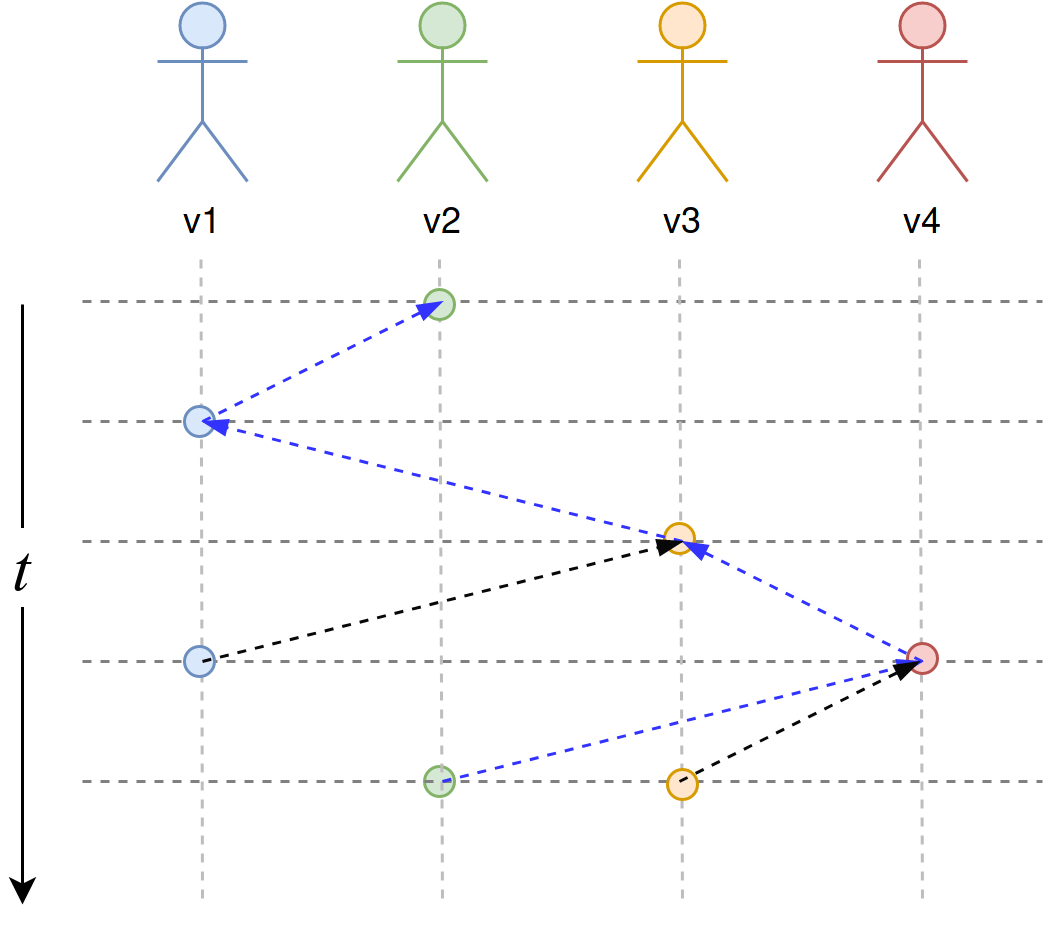
\includegraphics[width=0.8\columnwidth]{cbc-example}
  \captionsetup{justification=centering}
    \caption{\gls{cbc} blockchain example}
	\label{fig:example}
\end{figure}

\fig{fig:example} shows a small example of a \gls{cbc} execution
over a blockchain. Four nodes are pictured. Colored circles are messages sent by
validators, dotted arrows show their justifications. The selected blockchain is
depicted with blue arrows. It is obtained by running the \gls{ghost} algorithm
on the pictured view of the newtork, and would be the estimate of a new message
sent by an honest validator that has this view.

\fig{fig:example2} examplifies validator \(v_1\) producing a new message
and the resulting new blockchain. An honnest node includes all the latest
messages it has received (including its own last message). When a validator does
not include its own messages in its justification, it is considered as an
\textit{equivocator}, does not follow the protocol, and could be punished by
the network for such a behavior. Note that validator \(v_1\) does not equivovate
because its first message is in the justification of \(v_2\)'s first message,
and \(v_1\) has this message in the justification of its second message. It is
said that \(v_1\)'s first message is in the \textit{dependency} of its later
messages.

\begin{figure}[h]
	\centering
	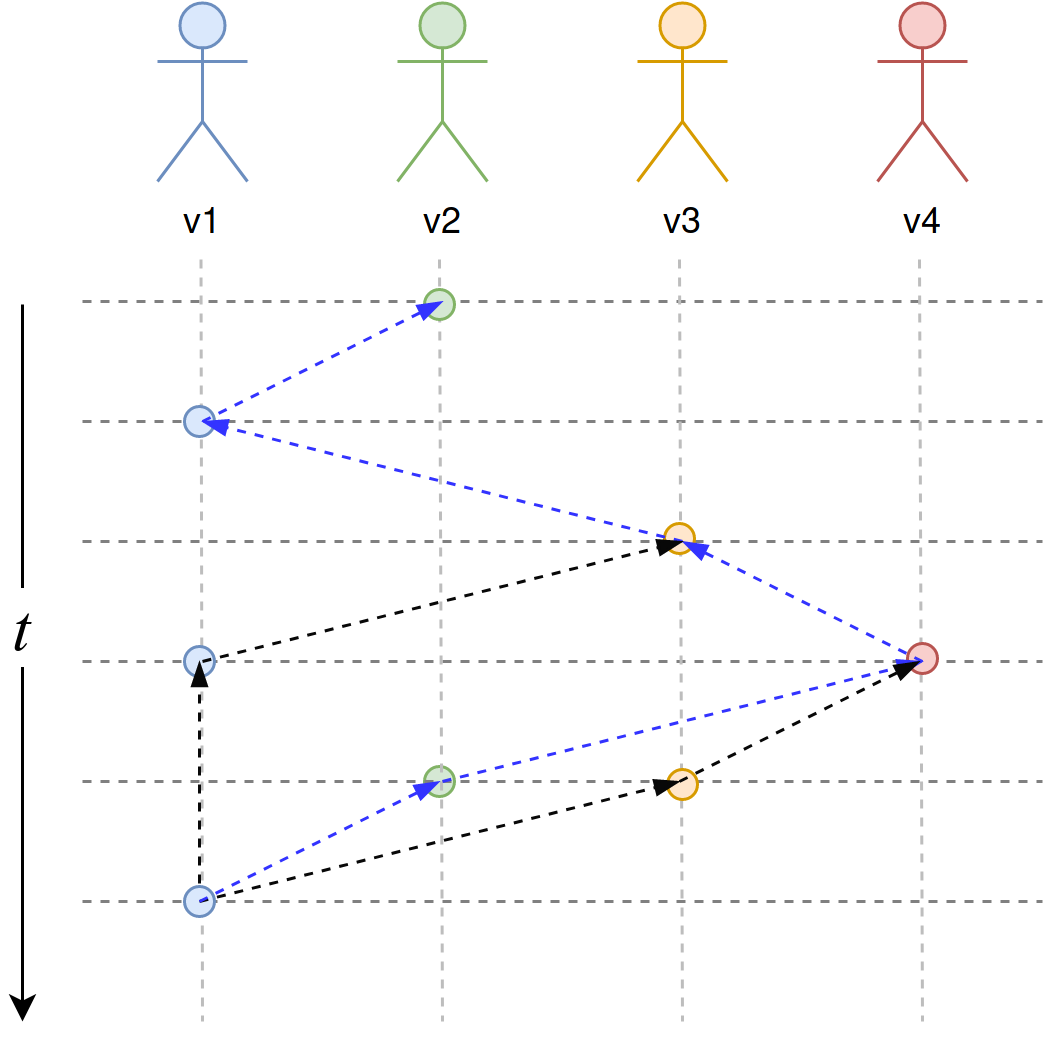
\includegraphics[width=0.8\columnwidth]{cbc-example-2}
  \captionsetup{justification=centering}
    \caption{\gls{cbc} blockchain example 2}
	\label{fig:example2}
\end{figure}

\todo{include a schema showing validators, justifications, estimates, \ldots in
more depth}

\todo{describe liveness, safety}
\todo{talk about finality, safety oracles, \ldots }
\todo{change structure; make comparison not between POS and POW but between POW
and CBC}
\FloatBarrier
\subsection{\gls{cbc} Casper vs \gls{pow}}
\label{ssec:powVsPos}

\subsubsection{Block production}
\todo{cite ref}
In a \gls{pow} setting, a miner can broadcast any block to the network, but the
block will only be picked up by the other nodes if it is valid. As the miner has
to work to produce a valid block, it cannot create blocks on the fly at any
time, whereas in a \gls{cbc} Casper setting, a node can broadcast blocks at any
time. 

\subsubsection{Timing assumption}
In a \gls{pow} protocol, the work a miner has to do to create a block is
parametrized by the difficulty of the cryptographic puzzle it has to solve. This
difficulty is set in such a way that it takes a certain time -on average- to
solve the puzzle. On the contrary, the \gls{cbc} Casper protocol family does not
make any timing assumption.

\subsubsection{Spam}
The two previous points imply that spamming issues are mitigated by the need to
work to produce blocks in a \gls{pow} chain. However, as there is a negligible
computational cost to produce Casper messages, a node could easily spam the
whole network.

\subsubsection{Economic majority}
\todo{cite ref, and better explanation}
As machines that are better at solving the cryptographic puzzle in a \gls{pow}
context are more expensive to buy and to operate, \todo{nah}
Economic majority is however built in the \gls{cbc} Casper protocol, in the form
of the weight that validators have.

\subsubsection{Building strategy}
In order to receive a reward for its work, a miner wants a block it has produced
to be included in the main chain. A \gls{pow} protocol usually states that the
chain with the most total difficulty is the main one. Therefore, a miner is
incentivised to build on top of the main chain. 
In a Casper setting, as there is no such incentive, a validator could build on
any chain, or even on its own chain.


\begin{table}[H]
    \centering{
        \begin{tabular}{|l|p{47mm}|p{47mm}|}
            \hline
            & \gls{pow} & \gls{cbc} Casper \\
            \hline
            Block production & Miners can publish blocks if the can prove they
            worked for it & Nodes can publish blocks at any time \\
            \hline
            Timing assumption & Work is a proxy for timing & None \\
            \hline
            Spam & Work removes the possibility to spam & Negligible
            computationnal costs to produce blocks imply potential spam \\
            \hline
            Economic majority & Work is a proxy for economic majority & Economic
            majority \\
            \hline
            Building strategy & Nodes are incentivised to build on the longest
            chain because they have to work to build blocks & No clear
            incentive to build on the longest chain \\
            \hline
        \end{tabular}
        \captionsetup{justification=centering}
        \caption{Summary of key differences between \gls{pow} and \gls{pos}}
        \label{fig:keyDiffPowPos}
    }
\end{table}

\section{Main problematic}
\todo{rename section}
As seen in \ssec{ssec:powVsPos}, many real-life implementation points are still
to define in order to have a practical \gls{cbc} Casper blockchain. One main
problem that arises is the selection of a block building strategy. This project
will try to propose a model to compare strategies, as well as a framework that
allows one to easily implement new strategies and discuss their performances
based on the proposed model.
Basic strategies that have predictable outputs will be implemented as well, in
order to validate the functionality of the framework.

\section{\texttt{core\_cbc}}
\texttt{core\_cbc} a Rust implementation of the \gls{cbc}-Casper, made by
TrueLevel \todo{introduce somewhere}. It implements the consensus algorithms proposed in the paper and
offers an abstract structure that can be used to create consensus on any value.

\section{Parity Ethereum}
\todo{remove redundancy in this chapter}
\todo{parity networking/gossiping layer research?}
Parity is a Rust Ethereum client. It includes a \textit{Pluggable Consensus}
module that allows one to easily add new consensus protocols by implementing an
interface.  At first, the goal of this project was to implement a small bridge
between the Parity module and the core cbc implementation to test block creation
strategies in a pseudo real-like manner. The implementation of the bridge was
not as straight forward as planned so it has been decided to cut it out and test
strategies without mimicking the network and client settings.

\subsection{Background work}
During the early stages of this project, a clear objective was set: to be able
to run a Casper \textit{testnet} with Parity custom nodes. Some work has been
done for the implementation of the \texttt{core-cbc} library into Parity, but
that was left to people that had a better understanding of the underlying
library. Furthermore, \todo{rephrase "a lot of"} a lot of effort had been
injected in the creation of a Docker infrastructure in order to easily deploy,
connect and monitor multiple custom Parity nodes on a single machine in order to
experiment with different message building strategies. The choice of using
Docker was made because there was a  possibility to work on the UniNE clusters,
which happen to work well with containerized software. After seeing that the
Parity implementation would take too much time to be completed, and therefore
might be unusable for this thesis, it has been decided to evaluate strategies
inside the \texttt{core-cbc} library instead of the more real-life-like setting
that is a Parity testnet. The main disadvantage of doing the experimentations in
the library is that the whole network latencies and topology are not taken into
account. However, a non-negligible advantage of implementing strategies in the
core library is that it will be easier to test them on consensus values that are
not only blockchains.  \todo{add that the lib was not fully tested at this point
and that further testing was needed before being able to test parity}

\subsection{Local testnet}
Scripts that create and manage two local nodes have been written. They launch 2
Parity instances with the \gls{cbc}-Casper consensus engine, and connect them
together. Each node has an user account to send transactions, as well as a
sender account, that can act as a validator in a Casper sense. Currently, each
node produces a block every 10 seconds. This is a basic strategy that enabled
further testing of the Parity inclusion of the \texttt{core-cbc}.

\subsection{Docker testnet}
Testing at a larger scale than two local instances was needed. The possibility
to access a cluster at the UniNE was discussed and the more straightforward way
to run programs on the cluster is to have containers. It was therefore decided
to create a more complex infrastructure using Docker containers.
\texttt{docker-compose} scripts were created to achieve this goal. An arbitrary
number of containers can be created at once and inter-connected in two different
ways:
\begin{itemize}
    \item fully connected;
    \item ring.
\end{itemize}

\begin{figure}
	\centering
	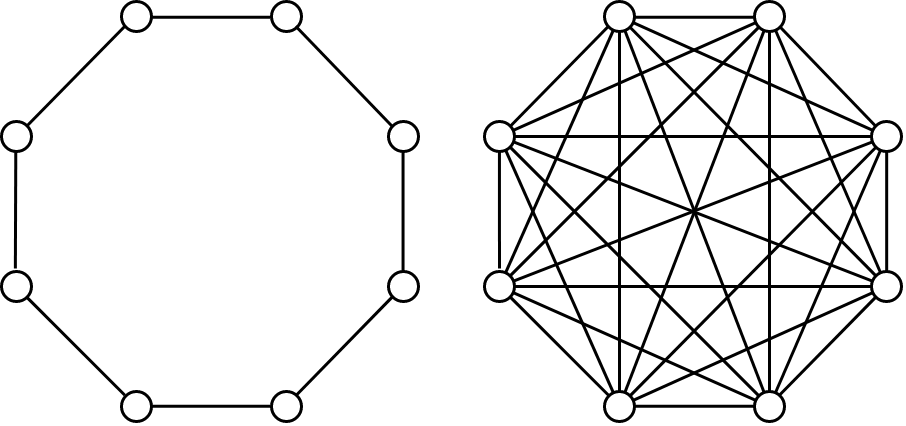
\includegraphics[width=0.8\columnwidth]{rings}
  \captionsetup{justification=centering}
    \caption{Parity nodes topologiess implemented in the Docker testnet. Ring
    layout (left), fully connected (right)}
	\label{fig:example2}
\end{figure}

The created nodes have the same types of accounts as for the local testnet.
\todo{include schemas of fully connected and ring layouts}
In the fully connected setting, each node is connected to every other node. In
the ring case, each node is connected to two other nodes in a circular manner.
Those were the two first layouts that were implemented for simplicity. It was
thought to add new layouts afterwards in order to match more precisely the real
network topology of the Ethereum \textit{mainnet}. However, because the Parity
implementation was deemed too time consuming to be used before the end of this
project, no further efforts have been put in that direction. Nevertheless, the
software architecture is in such a state than adding and removing topologies is
easily done through abstract structures.
